% Source: fixed PDF source-relative page 1 (printed page 306), Q12.
% Reproduces the source graph values and marks; tick labels are spaced for legibility.
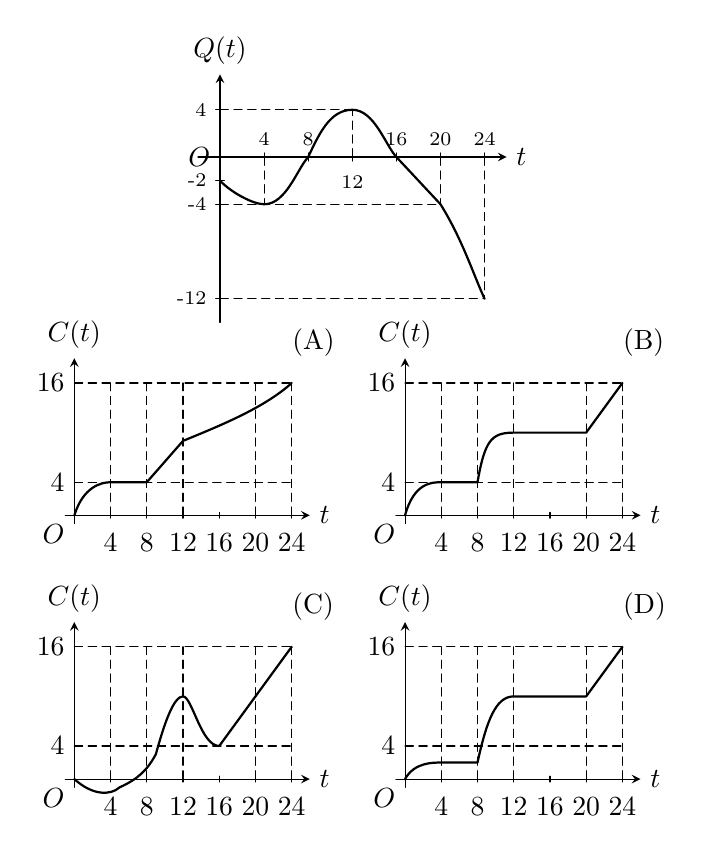
\begin{tikzpicture}[line cap=round,line join=round,>=stealth]
\tikzset{axis/.style={->,thin}, guide/.style={densely dashed,thin}, curve/.style={thick}}
% Daily temperature Q(t)
\begin{scope}[shift={(1.85cm,4.55cm)},x=0.14cm,y=0.15cm]
  \draw[axis] (0,-14)--(0,7) node[above] {$Q(t)$};
  \draw[axis] (-2,0)--(26,0) node[right] {$t$};
  \foreach \x in {4,8,16,20,24}{\draw (\x,0.35)--(\x,-0.35) node[above=2pt,font=\scriptsize] {\x};}
  \draw (12,0.35)--(12,-0.35) node[below=2pt,font=\scriptsize] {12};
  \foreach \y in {-12,-4,-2,4}{\draw (-0.4,\y)--(0.4,\y) node[left=3pt,font=\scriptsize] {\y};}
  \node[left] at (0,0) {$O$};
  \draw[guide] (0,-4)--(20,-4) (4,0)--(4,-4) (0,4)--(12,4) (12,0)--(12,4) (20,0)--(20,-4) (24,0)--(24,-12) (0,-12)--(24,-12);
  \draw[curve] (0,-2) .. controls (1,-3) and (3,-4) .. (4,-4)
    .. controls (6,-4) and (7,-1) .. (8,0)
    .. controls (9,2) and (10,4) .. (12,4)
    .. controls (14,4) and (15,1) .. (16,0)
    .. controls (18,-2) and (19,-3) .. (20,-4)
    .. controls (22,-7) and (23,-10) .. (24,-12);
\end{scope}
% Four candidate C(t) graphs
\def\optA{A}\def\optB{B}\def\optC{C}\def\optD{D}
\foreach \name/\dx/\dy in {A/0/0,B/4.2/0,C/0/-3.35,D/4.2/-3.35}{
  \begin{scope}[shift={(\dx,\dy)},x=0.115cm,y=0.105cm]
    \draw[axis] (0,-1)--(0,19) node[above] {$C(t)$};
    \draw[axis] (-1,0)--(26,0) node[right] {$t$};
    \foreach \x in {4,8,12,20,24}{\draw[guide] (\x,0)--(\x,16);}
    \foreach \y in {4,16}{\draw[guide] (0,\y)--(24,\y);}
    \node[left] at (0,4) {$4$}; \node[left] at (0,16) {$16$};
    \foreach \x in {4,8,12,16,20,24}{\draw (\x,0.35)--(\x,-0.35) node[below=2pt] {\x};}
    \node[below left] at (0,0) {$O$};
    \ifx\name\optA
      \draw[curve] (0,0) .. controls (1,3.5) and (3,4) .. (4,4)--(8,4)--(12,9)
        .. controls (16,10.8) and (21,13) .. (24,16);
    \fi
    \ifx\name\optB
      \draw[curve] (0,0) .. controls (1,4) and (3,4) .. (4,4)--(8,4)
        .. controls (8.8,9) and (9.5,10) .. (12,10)--(20,10)--(24,16);
    \fi
    \ifx\name\optC
      \draw[curve] (0,0) .. controls (2,-2) and (4,-2) .. (5,-1)
        .. controls (7,0) and (8,1) .. (9,3)
        .. controls (10,7) and (11,10) .. (12,10)
        .. controls (13,10) and (14,4) .. (16,4)--(24,16);
    \fi
    \ifx\name\optD
      \draw[curve] (0,0) .. controls (1,2) and (3,2) .. (4,2)--(8,2)
        .. controls (9,7) and (10,10) .. (12,10)--(20,10)--(24,16);
    \fi
    \node[above right] at (23,18) {(\name)};
  \end{scope}
}
\end{tikzpicture}
